\chapter{随机变量的数字特征}

\section{期望}

期望是集中趋势的一种刻画,定义 \ref{dfn:expectation and variance} 已经定义过
\begin{align}
	\E(X):=\begin{cases}
		\sum_{x\in\RR} xf(x),&\text{离散}\\[2ex]
		\int\iti xf(x)\d x,&\text{连续}
	\end{cases}
\end{align}
期望存在要求\textbf{绝对收敛}。
期望的一般定义
\[
	\E(X)=\int_0^1 x\d\CDF
\]
其中$\CDF$是CDF,这是一个Lebesque-Stieltjes积分。
\begin{theorem}{期望的性质}{}
	\begin{compactenum}
		\item 多元:$\E\bigfkh{(X_1,\ldots,X_n)}=\bigkh{\E(X_1),\ldots,\E(X_n)};$
		\item 函数:$\E\bigfkh{g(X_1,\ldots,X_n)}=\int_{\RR^n}g(x_1,\ldots,x_n)f(x_1,\ldots,x_n)\d x;$
		\item 线性:$\E(aX+bY)=a\E(X)+b\E(Y);$
		\item 若$X_1,\ldots,X_n$独立\footnote{后面很快会看到,有一个更弱的条件:$X_1,\ldots,X_n$不相关。},则$\E(X_1\cdots X_n)=\E(X_1)\cdots\E(X_n).$
	\end{compactenum}
\end{theorem}

\section{分位数、众数}

\begin{definition}{分位数}{quantile}
	定义$\forall\alpha\in(0,1)$若
	\[
		\P(X\leqslant a)\geqslant\alpha,\quad\P(X\geqslant a)\geqslant 1-\alpha,
	\]
	则称$a$为$X$的下$\alpha$-分位数(lower $\alpha$-quantile)。$a=\CDF\inv(\alpha)$。

\end{definition}
特别的,$\alpha=0.5$时,$a$对应中位数,也是集中趋势的一种刻画。

\paragraph{众数}众数也是一种集中趋势的刻画,方便定义$\arg\max f(x).$

\section{方差}

\dfnref{dfn:expectation and variance} 中已经定义过:
\begin{align}
	\Var(X):=\E\bigfkh{(X-\E(X))^2}\equiv\E(X^2)-\E^2(X)
\end{align}
标准差(standard deviation, SD) $\SD(X):=\sqrt{\Var(X)}.$

若$X$期望为$\mu$,标准差为$\sigma$,标准化
\begin{align}
	\check X:=\frac{X-\mu}{\sigma},
\end{align}
可使$\E(\check X)=0,\Var(\check X)=1.$
\begin{theorem}{方差的性质}{}
	\begin{compactenum}
		\item $\Var(c)=0,\enspace\Var(X+c)=\Var(X),\enspace\Var(cX)=c^2\Var(X);$
		\item $\Var(X+Y)=\Var(X)+\Var(Y)+2\Cov(X,Y);$
		\item $X,Y$独立时,可推出$\Var(X+Y)=\Var(X)+\Var(Y)$,\\
		$\Var(XY)=\Var(X)\Var(Y)+\underline{\E^2(X)\Var(Y)+\E^2(Y)\Var(X)}.$
	\end{compactenum}	
\end{theorem}
\begin{example}{期望在均方误差下的意义}{expectation under square error}
	期望是使得均方误差最小的常数估计,即$\forall c$均有
	\[
		\E\bigfkh{(X-c)^2}\geqslant\Var(X),
	\]
	取$=$当且仅当$c=\E(X)$。因为
	\begin{align*}
		\E\bigfkh{(X-c)^2}=\E(X^2)-2\E(X)c+c^2=:g(c)
	\end{align*}
	当且仅当$c=\E(X)$时取到$g_{\mathrm{min}}=\E(X^2)-\E^2(X)=\Var(X)$。
\end{example}
\begin{example}{中位数在绝对值误差下的意义}{}
	$m$为中位数,$\forall c$均有
	\[
		\E(|X-c|)\geqslant\E(|X-m|)
	\]
	取$=$当且仅当$c=m$。
\end{example}
\section{协方差及相关系数}
% 考虑随机变量$X,Y$
% \[
% 	\E(X)=\mu_1,\enspace\E(Y)=\mu_2,\enspace\Var(X)=\sigma_1^2,\enspace\Var(Y)=\sigma_2^2,
% \]
\begin{definition}{协方差}{covariance}
	定义协方差(covariance)
	\begin{align}
		\Cov(X,Y):=\E\bigfkh{(X-\E(X))(Y-\E(Y))}\equiv\E(XY)-\E(X)\E(Y).
	\end{align}
	显然,$\Cov(X,X)=\Var(X)$。
\end{definition}
协方差是可交换且双线性的。

\begin{definition}{协方差矩阵}{covariance matrix}
	定义$X=(X_1,\ldots,X_n),Y=(Y_1,\ldots,Y_n)$的协方差矩阵(covariance matrix)
	\begin{align}
		\Cov(X,Y):=\begin{bmatrix}
			\Cov(X_i,Y_j)
		\end{bmatrix}_{n\times n},
	\end{align}
	相应的,$\Cov(X,X)$就是向量$X$的方差矩阵。
\end{definition}
由协方差矩阵可以得到
\begin{align}
	\Var\biggkh{\sum_{i=1}^nX_i}=\sum_{i=1}^n\Var(X_i)+2\sum_{i<j}\Cov(X_i,X_j)\equiv\sum_{i,j}\Cov(X_i,X_j).
\end{align}
\begin{example}{多项分布的协方差}{covariance of multinomial distribution}
	在\exmref{exm:multinomial distribution} 中给过多项分布$(X_1,\ldots,X_n)\sim\Bern(n,p_1,\ldots,p_n)$,显然,其边际分布$X_i\sim\Bern(n,p_i)$,下面给出$X_i,X_j$的协方差
	\[
		\Cov(X_i,X_j)=-np_ip_j,\quad i\neq j.
	\]
	得到这个结论的过程见条件期望部分的\exmref{exm:covariance of multinomial distribution 2}。
\end{example}
\begin{example}{配对问题的期望和方差}{}
	尽管\exmref{exm:weak dependence condition} 中$X$的分布列较复杂,我们依然可以通过简单的计算得到其期望和方差。
	
	记$X_i\sim\Bern\bigkh{\P(A_i)}$表示第$i$个人是否拿到自己的帽子,从而
	\[
		X=X_1+\cdots+X_n,
	\]
	尽管$X_i$间并不独立,但其期望是相同的($1/n$)。
	进而可以得到$X$的期望就是期望的和(这并不要求独立性)
	\[
		\E(X)=\sum_{i=1}^n\E(X_i)=n\cdot\frac1n=1.
	\]
	而$X_iX_j(i\neq j)$的期望
	\[
		\E(X_iX_j)=\P(X_iX_j=1)+0=\frac1n\cdot\frac1{n-1},
	\]
	从而协方差
	\begin{align*}
		\Cov(X_i,X_j)&=\E(X_iX_j)-\E(X_i)\E(X_j)\\
		&=\frac1n\cdot\frac1{n-1}-\frac1n\cdot\frac1n=\frac1{n^2(n-1)}.
	\end{align*}
	因此方差
	\begin{align*}
		\Var(X)&=\sum_{i=1}^n\Var(X_i)+\sum_{i\neq j}\Cov(X_i,X_j)\\
		&=n\cdot\frac1n\kh{1-\frac1n}+n(n-1)\cdot\frac1{n^2(n-1)}=1.
	\end{align*}
\end{example}
\begin{definition}{相关系数}{correlation coefficient}
	定义相关系数(correlation coefficient)
	\begin{align}
		\Corr(X,Y):=\frac{\Cov(X,Y)}{\sqrt{\Var(X)\Var(Y)}}\equiv\E\biggkh{\frac{X-\E(X)}{\sqrt{\Var(X)}},\frac{Y-\E(Y)}{\sqrt{\Var(Y)}}},
	\end{align}
	若$\Corr(X,Y)=0$,称为$X,Y$不(线性)相关。
\end{definition}
$X,Y$不相关与
\[
	\E(XY)=\E(X)\E(Y),\quad\Var(X+Y)=\Var(X)+\Var(Y).
\]
是等价的。易见,独立是不相关的充分不必要条件。
\begin{theorem}{相关系数的性质}{}
	$\abs{\Corr(X,Y)}\leqslant 1$,取等号当且仅当
	\[
		\P(Y=aX+b)=1,\enspace(\text{almost~surely,~a.}\,\text{s.})
	\]
	只需考虑Cauchy-Schwartz不等式\index{a. s.,以概率1}
	\begin{align}
		\E^2(UV)\leqslant\E(U)\E(V),
	\end{align}
	这可以用$\forall t\in\RR,\E\bigfkh{(U-tV)^2}\geqslant 0$证明。
\end{theorem}
\begin{example}{二元正态分布的相关系数}{correlation coefficient of 2-D normal distribution}
	取$\xi:=\frac{x-\mu_1}{\sigma_1},\eta:=\frac{y-\mu_2}{\sigma_2}$,则
	\begin{align*}
		\Corr(X,Y)%&=\frac1{2\pi\sqrt{1-\rho^2}}\iint_{\RR^2}\xi\eta\exp\biggfkh{-\frac{\xi^2+\eta^2-2\rho\xi\eta}{2(1-\rho^2)}}\d\xi\nd\eta\\
		&=\frac1{2\pi\sqrt{1-\rho^2}}\iint_{\RR^2}\xi\eta\exp\biggfkh{-\frac{(\xi-\rho\eta)^2}{2(1-\rho^2)}-\frac{\eta^2}2}\d\xi\nd\eta
	\end{align*}
	由
	\[
		\int\iti x\e{-a(x-b)^2+c}\d x=\sqrt{\frac\pi{a}}b\e c.
	\]
	可得
	\begin{align*}
		\Corr(X,Y)&=\frac1{2\pi\sqrt{1-\rho^2}}\int\iti\eta\sqrt{2\pi(1-\rho^2)}\cdot\rho\eta\e{-\eta^2/2}\d\eta\\
		&=\frac\rho{\sqrt{2\pi}}\int\iti\eta^2\e{-\eta^2/2}\d\eta=\rho.
	\end{align*}
\end{example}
\section{矩}
\begin{definition}{矩}{moment}
	$X$的关于$c$点的$k$阶矩(moment)
	\begin{align}
		\E\bigfkh{(X-c)^k},
	\end{align}
	特别的,当$c=0$时,称为原点矩;当$c=\E(X)$时,称为中心矩。
\end{definition}
故$\E(X)$为1阶原点矩,$\Var(X)$为2阶中心矩。
\begin{definition}{偏度系数}{skewness}
	定义3阶标准矩为偏度系数(skewness)
	\begin{align}
		\mathrm{skew}(X):=\E\biggfkh{\Bigkh{\frac{X-\mu}\sigma}^3}.
	\end{align}
\end{definition}
1阶标准矩为0,2阶标准矩为1。当中心往右偏时,偏度系数$<0$。
\begin{definition}{峰度系数}{kurtosis}
	定义4阶标准矩为峰度系数(kurtosis)
	\begin{align}
		\mathrm{kurt}(X):=\E\biggfkh{\Bigkh{\frac{X-\mu}\sigma}^4}.
	\end{align}
\end{definition}
正态分布的峰度系数为3%,以正态分布为标准,定义超额峰度系数=峰度系数$-~3$
。一般的,尖峰厚尾的峰度系数$>3$。
\section{矩母函数}
\begin{definition}{矩母函数}{moment generating funtion}
	若下面期望在$t$的某含0邻域内存在,
	\begin{align}\label{MGF def}
		\MGF_X(t):=\E\kh{\e{tX}}
	\end{align}
	则称$\MGF_X(t)$为$X$的矩母函数(moment generating function, MGF).\index{MGF, 矩母函数}
\end{definition}
矩母函数的意义是用来确定矩
\begin{align}
	\E(X^n)=\MGF_X^{(n)}(0)
\end{align}
\begin{example}{指数分布和正态分布的矩母函数}{MGF of Expo & Norm}
	若$X\sim\Expo(\lambda)$,则 
	\[
		\MGF_X(t)=\int\zti\e{tx}\lambda\e{-\lambda x}\d x=\frac\lambda{\lambda-t},\quad t\in(-\lambda,\lambda).
	\]
	\tcblower
	若$X\sim\Norm(\mu,\sigma^2)$,则
	\[
		\MGF_X(t)=\frac1{\sqrt{2\pi}\sigma}\int\iti\e{tx}\e{-(x-\mu)^2/2\sigma^2}\d x=\exp\Bigkh{\mu t+\frac12\sigma^2t^2}.
	\]
	特别的,若$X\sim\Norm(0,1)$,则 
	\[
		\MGF_X(t)=\e{-t^2/2}=\sum_{n=0}^\infty\frac{(2n)!}{2^nn!}\frac{t^{2n}}{(2n)!}.
	\]
	故$\E(X^{2k+1})=0,\enspace\E(X^{2k})=(2k-1)!!$
\end{example}
\begin{theorem}{矩母函数确定分布}{}
	若存在$a>0$,使得
	\[
		\MGF_X(t)=\MGF_Y(t),\quad\forall t\in(-a,a)
	\]
	则$X,Y$同分布。
\end{theorem}
证明超过了本节课的范围。
\begin{example}{离散分布的矩母函数}{}
	从$X$的矩母函数,比如
	\[
		\MGF_X(t)=\frac14\e{-t}+\frac12+\frac18\e{4t}+\frac18\e{5t},
	\]
	可直接看出$X$的分布列。
	\iffalse
	\begin{center}
		\begin{tabular}{ccccc}
			\toprule
			$X$&$-1$&0&4&5\\
			\midrule
			$p$&$\frac14$&$\frac12$&$\frac18$&$\frac18$\\
			\bottomrule
		\end{tabular}
	\end{center}
	\fi
\end{example}
\begin{example}{同矩不一定同分布}{}
	对数正态分布$\ln X_1\sim\Norm(0,1)$,则$X_1$的PDF
	\[
		f_1(x)=\frac1{\sqrt{2\pi}x}\e{-\ln^2x/2},\quad x>0
	\]
	构造$X_2$,其PDF
	\[
		f_2(x)=f_1(x)\bigfkh{1+\sin(2\pi\ln x)}\geqslant 0.
	\]

	可以证明,$X_1,X_2$所有的矩均相等
	\[
		\E(X_2^n)=\E(X_1^n)+\int\zti x^nf_1(x)\sin(2\pi\ln x)\d x
	\]
	后面的积分做换元$y:=\ln x-n$可积得结果为0.
\end{example}
从上面构造的例子可以看出:同矩不一定同分布,因此矩母函数相同是比所有矩相同更强的条件。
\begin{theorem}{独立随机变量和的分布}{the distribution of the sum of the independent random variable}
	若$X,Y$独立,则
	\[
		\MGF_{X+Y}(t)=\MGF_X(t)\MGF_Y(t).
	\]
	%\prf \MGF_{X+Y}(t)=\E(\e{tX}\e{tY})=\E(\e{tX})\E(\e{tY})=\MGF_X(t)\MGF_Y(t).\rqed
\end{theorem}
因此,$n$个独立的正态分布$X_i\sim\Norm(\mu_i,\sigma_i^2)$的和仍然服从正态分布,且
\[
	\sum_{i=1}^nX_i\sim\Norm\kh{\sum_{i=1}^n\mu_i,\sum_{i=1}^n\sigma_i^2}.
\]
\begin{definition}{联合分布的矩母函数}{}
	联合分布的矩母函数定义为
	\begin{align}
		\MGF_{X_1,\ldots,X_n}(t_1,\ldots,t_n):=\E\kh{\e{t_1X_1+\cdots+t_nX_n}}.
	\end{align}
\end{definition}
也可以通过矩母函数确定分布。
\begin{definition}{概率母函数}{probability generating function}
	离散型随机变量$X$取值为非负整数
	\[
		p_k=\P(X=k),\quad k=0,1,2,\ldots
	\]
	则概率母函数(probability generating function, PGF)\index{PGF, 概率母函数}
	\[
		g(t):=\E(t^X)=\sum_{k=0}^\infty t^kp_k.
	\]
\end{definition}
概率母函数给出了各点的概率
\[
	\P(X=k)=\frac{g^{(k)}(0)}{k!}
\]
也给出了期望$\E(X)=g'(1)$.
\begin{definition}{特征函数}{characteristic function}
	定义特征函数(characteristic function, CF)\index{CF, 特征函数}
	\begin{align}\label{CF-def}
		\psi(t):=\E\kh{\e{\i tX}}.
	\end{align}
\end{definition}
与矩母函数不同,特征函数总是存在的。
\section{条件期望}
\begin{definition}{条件期望}{conditional expectation}
	定义条件期望
	\begin{align}
		\E(Y|X\in A):=\begin{cases}
			\sum_i y_i\P(Y=y_i|X\in A),&\text{离散}\\
			\int_\RR yf(y|X\in A)\d y,&\text{连续}
		\end{cases}
	\end{align}
	若$\P(X\in A)>0$,条件期望可由下式计算
	\begin{align}
		\E(Y|X\in A)=\frac{\E(Y,X\in A)}{\P(X\in A)}.
	\end{align}
\end{definition}
$\E(Y|X)$是$X$的函数,是一个新的随机变量($Y$对$X$的回归函数)。
\begin{example}{二元正态分布的条件期望}{}
	$(X,Y)\sim\Norm(\mu_1,\mu_2,\sigma_1^2,\sigma_2^2,\rho)$,由\exmref{exm:conditional PDF of 2-D normal distribution}
	\[
		\E(Y|X)=\mu_2+\rho\frac{\sigma_2}{\sigma_1}(X-\mu_1)^2.
	\]
\end{example}
\begin{theorem}{全期望公式}{}
	可由全概率公式推出
	\begin{align}
		\E(Y)=\E\bigfkh{\E(Y|X)}.
	\end{align}
\end{theorem}
\begin{theorem}{条件期望的性质}{}
	\begin{compactenum}
		\item $\E\bigfkh{g(X)h(Y)|X}=g(X)\E\bigfkh{h(Y)|X}$;
		\item $\E\bigfkh{\E\bigfkh{g(X,Y)|X}}=\E\bigfkh{g(X,Y)}$;
		\item 若$X,Y$独立,则$\E(Y|X)=\E(Y)$为常数,与$X$无关。
	\end{compactenum}
\end{theorem}
注意第3条,若$\E(Y|X)=\E(Y)$,则$X,Y$不相关:
\[
	\E(XY)=\E\bigfkh{\E(XY|X)}=\E\bigfkh{X\E(Y|X)}=\E\bigfkh{X\E(Y)}=\E(X)\E(Y).
\]
推不出$X,Y$独立。
\begin{example}{多项分布的协方差}{covariance of multinomial distribution 2}
	接\exmref{exm:covariance of multinomial distribution},由全期望公式
	\[
		\E(X_iX_j)=\E\bigfkh{\E(X_iX_j|X_j)}=\E\bigfkh{X_j\E(X_i|X_j)}.
	\]
	而$\E(X_i|X_j)$可以理解成先从$n$份中抽出$X_j$个$B_j$,剩下变成新的多项分布
	\[
		(\ldots,X_i,\ldots)_{i\neq j}\sim\Bern\Bigkh{n-X_j,\ldots,\frac{p_i}{1-p_j},\ldots}_{i\neq j}
	\]
	继而
	\begin{gather*}
		\E(X_i|X_j)=(n-X_j)\frac{p_i}{1-p_j}.\\
		\begin{aligned}
			\E(X_iX_j)&=\frac{p_i}{1-p_j}\bigfkh{n\E(X_j)-\E(X_j^2)}\\
			&=\frac{p_i}{1-p_j}\bigfkh{n\cdot np_j-\bigkh{np_j(1-p_j)+(np_j)^2}}\\
			&=n(n-1)p_ip_j.
		\end{aligned}
	\end{gather*}
	协方差
	\[
		\Cov(X_i,X_j)=n(n-1)p_ip_j-np_i\cdot np_j=-np_ip_j.
	\]
\end{example}
\begin{theorem}{最优预测}{}
	用$g(X)$估计$Y$的均方误差
	\begin{align}
		\E\bigfkh{(Y-g(X))^2}\geqslant\E\bigfkh{(Y-\E(Y|X))^2}.
	\end{align}
\end{theorem}
这源于\exmref{exm:expectation under square error} 所给出的:
\[
	\E\bigfkh{(Y-g(X))^2|X}\geqslant\E\bigfkh{(Y-\E(Y|X))^2|X}.
\]
事实上这也给出了条件期望$\E(Y|X)$的几何意义:$Y$在$X$张成的线性空间上的投影。
\begin{example}{误差}{error}
	$Y$对$X$的回归函数$\hat Y:=\E(Y|X)$,误差$\tilde Y:=Y-\hat Y$,易得
	\[
		\E(\hat Y)=\E(Y),\quad\E(\tilde Y)=0,
	\]
	且$\hat Y,\tilde Y$不相关,也就是说
	\[
		\Var(Y)=\Var(\hat Y)+\Var(\tilde Y).
	\]
	\begin{center}
		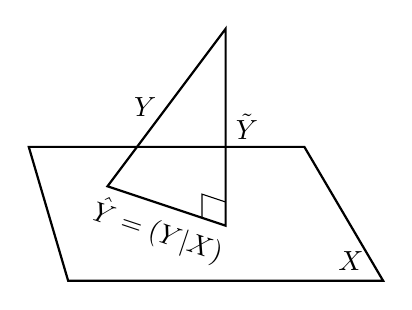
\begin{tikzpicture}
			\draw[thick](0, 0)--(1.5, 2)node[midway, left]{$Y$}--(1.5, -.5)node[midway, right]{$\tilde Y$}--cycle node[midway, sloped, below]{$\hat Y=\E(Y|X)$};
			\draw(1.2, -.4)--(1.2, -.1)--(1.5, -.2);
			\draw[thick](-1, .5)--(2.5, .5)--(3.5, -1.2)node[above left]{$X~$}--(-.5, -1.2)--cycle;
		\end{tikzpicture}
		\captionof{figure}{$Y,\hat Y,\tilde Y$关系示意图}
	\end{center}
\end{example}
\begin{definition}{条件方差}{conditional variance}
	定义条件方差
	\begin{align}
		\Var(Y|X):=\E\bigfkh{\bigkh{X-\E(Y|X)}^2|X}
	\end{align}
\end{definition}
自然
\begin{align}
	\Var(Y|X)=\E(Y^2|X)-\E^2(Y|X).
\end{align}
\begin{theorem}{全方差公式}{}
	由\exmref{exm:error}
	\begin{align}
		\Var(Y)=\E\bigfkh{\Var(Y|X)}+\Var\bigfkh{\E(Y|X)}.
	\end{align}
\end{theorem}
\begin{example}{随机变量个随机变量的和}{}
	随机变量序列$X_1,X_2,\ldots$ iid,$N$是取值为正整数的随机变量,且与$X_i$独立,令$Y=X_1+\cdots+X_N$,则
	\begin{align}
		\E(Y)&=\E\bigfkh{\E(Y|N)}=\E\bigfkh{N\E(X)}=\E(N)\E(X);\\\notag
		\Var(Y)&=\E\bigfkh{\Var(Y|N)}+\Var\bigfkh{\E(Y|N)}\\\notag
		&=\E\bigfkh{N\Var(X)}+\Var\bigfkh{N\E(X)}\\
		&=\Var(X)\E(N)+\E^2(X)\Var(N).
	\end{align}
	特别的,$N\sim\Pois(\lambda)$时,称$Y$为复合Poisson随机变量
	\[
		\Var(Y)=\lambda\bigfkh{\Var(X)+\E^2(X)}=\lambda\E(X^2).
	\]
\end{example}